\documentclass{llncs}
\usepackage{ amssymb }
\usepackage[linesnumbered, ruled, vlined]{algorithm2e}
\usepackage{tikz}
\usetikzlibrary{arrows,shapes,positioning}
\usepackage{subcaption}
\captionsetup{compatibility=false}


\usepackage{xcolor}
\definecolor{todocolor}{RGB}{72,130,84}
\newcommand{\todo}[1] {
  \textcolor{todocolor}{TODO: #1}
}

\usepackage{ntheorem}
\newtheorem{observation}{Observation}
\renewcommand{\theobservation}{\arabic{observation}.}% #.

\newcommand{\bfalg}{\texttt{\small{IVC\_BF}}}
\newcommand{\ucalg}{\texttt{\small{IVC\_UC}}}
\newcommand{\ucbfalg}{\texttt{\small{IVC\_UCBF}}}
\newcommand{\mustalg}{\texttt{\small{IVC\_MUST}}}
\newcommand{\getivc}{\textsc{GetIVC}}
\newcommand{\mike}[1]{\textcolor{red}{Mike: #1}}


\begin{document}

\title{Online Enumeration of All Minimal Inductive Validity Cores}

\author{Jaroslav Bend\'ik\inst{1}
	\and Elaheh Ghassabani\inst{2}
	\and Michael Whalen\inst{2}
	\and Ivana \v Cern\'a\inst{1}
}

\institute{Faculty of Informatics, Masaryk University, Brno, Czech Republic\\
\email{\{xbendik,cerna\}@fi.muni.cz}
\and
Department of Computer Science \& Engineering, University of Minnesota, MN, USA\\
\email{\{ghass013,mwwhalen\}@umn.edu}
}


\maketitle
\begin{abstract}
Symbolic model checkers can construct proofs of safety properties over complex models, but when a proof succeeds, the results do not generally provide much insight to the user.  Minimal Inductive Validity Cores (MIVCs) trace a property to a minimal set of model elements necessary for constructing a proof, and can help to explain why a property is true of a model.  In addition, the traceability information provided by MIVCs can be used to perform a variety of engineering analysis such as coverage analysis, robustness analysis, and vacuity detection.  The more MIVCs are identified, the more precisely such analyses can be performed.   Nevertheless, a full enumeration of all MIVCs is in general intractable due to the large number of possible model element sets.  The bottleneck of existing algorithms is that they are not guaranteed to emit minimal IVCs until the end of the computation, so returned results are not known to be minimal until all solutions are produced.

In this paper, we propose an algorithm that identifies MIVCs in an \emph{online} manner (i.e., one by one) and can be terminated at any time.  We benchmark our new algorithm against existing algorithms on a variety of examples, and demonstrate that our algorithm not only is better in intractable cases but also completes the enumeration of MIVCs faster than competing algorithms in many tractable cases.

\keywords{Inductive Validity Cores, SMT-based model checking, Inductive proofs, Traceability, Proof cores}
\end{abstract}



\section{Introduction}
\label{sec:intro}
Symbolic model checking using induction-based techniques such as IC3/PDR~\cite{Een2011:PDR}, $k$-induction~\cite{SheeranSS00}, and $k$-liveness~\cite{conf/fmcad/ClaessenS12} can be used to determine whether properties hold of complex finite or infinite-state systems.  Such tools are popular both because they are highly automated (often requiring no user interaction other than the specification of the model and desired properties), and also because, in the event of a violation, the tool provides a counterexample demonstrating a situation in which the property fails to hold.  These counterexamples can be used both to illustrate subtle errors in complex hardware and software designs~\cite{hilt2013,McMillan99:compositional,Miller10:CACM} and to support automated test case generation~\cite{Whalen13:OMCDC,You15:dse}.

If a property is proved, however, most model checking tools do not provide additional information.  This can lead to situations in which developers have an unwarranted level of confidence in the behavior of the system.  Issues such as vacuity~\cite{Kupferman03:Vacuity}, incorrect environmental assumptions~\cite{Whalen07:FMICS}, and errors either in English language requirements or formalization~\cite{Pike06:axioms} can all lead to failures of ``proved'' systems.  Thus, even if proofs are established, one must approach verification with skepticism.

Recently, {\em proof cores}~\cite{jasper_gold} have been proposed as a mechanism to determine which elements of a model are used when constructing a proof.  This idea is formalized by Ghassabani et al. for inductive model checkers~\cite{Ghass16} as {\em Inductive Validity Cores} (IVCs). IVCs offer proof explanation as to why a property is satisfied by a model in a formal and human-understandable way.  The idea lifts UNSAT cores~\cite{zhang2003extracting}
to the level of sequential model checking algorithms using induction.  Informally, if a model is viewed as a conjunction of constraints,
a minimal IVC (MIVC) is a set of constraints that is sufficient to construct a proof such that if any constraint is removed, the property is no longer valid.  
%
Depending on the model and property to be analyzed, there are many possible MIVCs, and there is often substantial diversity between the IVCs used for proof.  

In previous work~\cite{Ghass16,Murugesan16:renext,Ghass17Cov,Ghass17AllIVCs} we have explored several different uses of IVCs, including: 

\noindent \textbf{Traceability: } For functional properties that can be proven with inductive model checkers, inductive validity cores can provide accurate traceability matrices with no user effort.  Given multiple IVCs, {\em rich traceability} matrices~\cite{Murugesan16:renext} can be automatically constructed that provide additional insight about {\em required} vs. {\em optional} design elements.

\noindent \textbf{Vacuity detection:} The idea of syntactic vacuity detection (checking whether all subformulae within a property are necessary for its validity) has been well studied~\cite{Kupferman03:Vacuity}.   IVCs allow a generalized notion of vacuity that can indicate weak or mis-specified properties even when a property is syntactically non-vacuous.

\noindent \textbf{Coverage analysis:} Closely related to vacuity detection is the idea of {\em coverage analysis}, e.g., are all atoms in the model necessary for at least one of the properties proven about the model?  Several different notions of coverage have been proposed~\cite{chockler_coverage_2003,kupferman_theory_2008}, but these tend to be very expensive to compute.

\noindent \textbf{Impact Analysis:} Given a single (or for more accurate results, all) MIVCs, it is possible to determine which requirements may be falsified by changes to the model.  This analysis allows for selective regression verification of tests and proofs: if there are alternate proof paths that do not require the modified portions of the model, then the requirement does not need to be re-verified.

\noindent \textbf{Design Optimization:} Synthesis tools can benefit from MIVCs in the process of transforming an abstract behavior into a design implementation. A practical way of calculating all MIVCs allows synthesizers to find a minimum set of design elements (optimal implementation) for a certain behavior. Such optimizations can be performed at different levels of synthesis.

To be useful for these tasks, the generation process must be efficient and the generated IVC must be accurate and precise (that is, sound and minimal).  In previous work, we have developed an efficient {\em offline} algorithm~\cite{Ghass17AllIVCs} for finding all minimal IVCs based on the MARCO algorithm for MUSes~\cite{marco2016fast}.  The algorithm is considered {\em offline} because it is not until all IVCs have been computed that one knows whether the solutions computed are, in fact, minimal.  In cases in which models contain many IVCs, this approach can be impractically expensive or simply not terminate.

In this paper, we propose a novel {\em online} algorithm for MIVC enumeration.  With this algorithm, solutions are produced at a regular rate, and each solution produced is guaranteed to be minimal.  Additionally, for models with a large number of IVCs, the proposed algorithm is considerably more efficient than the baseline MARCO algorithm.  We demonstrate this via an experimental evaluation.

The rest of the paper is organized as follows. In Section~\ref{sec:preliminaries} we define all the necessary notions. Section~\ref{sec:existing-techniques} summarizes the existing techniques. In Section~\ref{sec:algorithm} we present our novel algorithm. Section~\ref{sec:example-execution} provides an example execution of our algorithm. Finally, sections \ref{sec:implementation} and \ref{sec:experiment} cover implementation details and present experimental results. 	




%\section{Motivating Example}
%\label{sec:mot-example}
%\input{motivation}
%\todo{Mike and Elaheh: Do we need a motivating example? Something like altitude switch model in your all ivcs paper. Currently, there is just a very brief preliminaries section. It might be unclear for the reader how does the transition system looks like.}

\section{Preliminaries}
\label{sec:preliminaries}
A transition system $(I,T)$ over a state space $S$ consists of an initial state predicate $I : S \rightarrow bool$ and a transition step predicate $T : S \times S \rightarrow bool$. The notion of reachability for $(I, T)$ is defined as the smallest predicate $R : S \rightarrow bool$ satisfying the following formulae:

\begin{itemize}
	\item[] $\forall s \in S: \, I(s) \Rightarrow R(s)$
	\item[] $\forall s, s' \in S: \, R(s) \wedge T(s, s') \Rightarrow R(s')$
\end{itemize}

A safety property $P: S \rightarrow bool$ holds on a transition system $(I, T)$ iff it holds on all reachable states, i.e., $\forall s \in S: \, R(s) \Rightarrow P(s)$. We denote this by $(I, T) \vdash P$. We assume
the transiton step predicate $T$ is equivalent to   a conjunction of transition step predicates $T_1, \ldots, T_n$,  called top level conjuncts. 
%the transition relation has the structure of a top-level conjunction $T(s, s') = T_1(s, s') \wedge \cdots \wedge T_n(s, s')$. 
In such case, $T$ can be identified with the set of its top level conjuncts $\{ T_1, \ldots, T_n\}$. By further abuse of notation, we write $T \setminus \{ T_i \}$ to denote removal of top level conjunct $T_i$ from $T$, and $T \cup \{ T_j\}$ to denote addition of top level conjunct $T_j$ to $T$. 


\begin{definition}
A set of conjucnts $U \subseteq T$ is an Inductive Validity Core (IVC) for $(I, T) \vdash P$ iff $(I, U) \vdash P$. Moreover, $U$ is a Minimal IVC (MIVC) for $(I, T) \vdash P$ iff $(I, U) \vdash P$ and $\forall U_i \in U: \, (I, U \setminus \{ U_i\}) \nvdash P$.
\end{definition}

Note, that the minimality is with respect to the set inclusion and not wrt cardinality. There can be multiple MIVCs with different cardinalities. 

%\textit{concept used here is set minimality, not minimum cardinality. This means, that there can be multiple MIVCs with different cardinalities.} 

\todo{Example}







\section{Existing Techniques}
\label{sec:existing-techniques}
\newcommand{\fUnex}{f_{\mathit{Unexplored}}}
%Let us first consider
Consider first
a naive enumeration algorithm that   explicitly checks each subset of $T$ for being an IVC  and then finds the minimal IVCs  using subset inclusion relation. The main disadvantage of this approach is the large number of checks since there are exponentially many subsets of $T$.
We briefly describe existing techniques that can be used to find all MIVCs while checking only a a small portion of subsets of $T$  for being IVCs.  Most of the techniques were inspired by the MUS enumeration techniques~\cite{Liffiton2016,bacchus2015using,belov2012muser2,nadel2014accelerated,DBLP:conf/sefm/BendikBBC16,DBLP:conf/fsttcs/BendikBCB16}   proposed in the area of constraint processing and applied by Ghassabani et al.~\cite{Ghass17AllIVCs,Ghass16}.


\begin{definition}[Inadequacy] A set of conjuncts  $U \subseteq T$  is an \emph{inadequate} set for $(I, T) \vdash P$ iff $(I, U) \nvdash P$. Especially, $U \subseteq T$ is a \emph{Maximal Inadequate Set (MIS)} for $(I, T) \vdash P$ iff $U$ is inadequate and $\forall T_i \in (T \setminus U): \, (I, U \cup \{ T_i\}) \vdash P$.
\end{definition}

Inadequate sets are duals to inductive validity cores. Each $U \subseteq T$ is either inadequate set or an inductive validity core. In order to unify the notation, we   use notation \emph{inadequate} and \emph{adequate}. Note that especially minimal inductive validity cores can be thus called  minimal adequate sets.



The first property used to improve the naive enumeration algorithm is the \emph{monotonicity} of  adequacy   with respect to the subset inclusion.

\begin{lemma}[Monotonicity]
\label{lemma:monotonicity}
If a set of conjuncts  $U \subseteq T$  is an adequate set for $(I, T) \vdash P$   than all its supersets are adequate for  $(I, T) \vdash P$ as well:
\begin{center}
$\forall U_1 \subseteq U_2 \subseteq T: \, (I, U_1) \vdash P \Rightarrow (I, U_2) \vdash P$.
\end{center}
Symmetrically, if   $U \subseteq T$  is an inadequate set for $(I, T) \vdash P$   than all its subsets are inadequate for  $(I, T) \vdash P$ as well:
\begin{center}
$\forall U_1 \subseteq U_2 \subseteq T: \, (I, U_2) \nvdash P \Rightarrow (I, U_1) \nvdash P$.
\end{center}
\end{lemma}

\begin{proof}
%From $U_1 \subseteq U_2$ we have $U_2 \Rightarrow U_1$. Thus the
If $U_1 \subseteq U_2$ then reachable states of $(I, U_2)$ form  a subset of the reachable states
of $(I, U_1)$.
\end{proof}
%
%\begin{corollary}
%For $(I, T) \vdash P$, if $U \subseteq T$ is inadequate for property $P$, than all of its subsets are inadequate for $P$ as well:
%\begin{center}
%$\forall U_1 \subseteq U_2 \subseteq T: \, (I, U_2) \nvdash P \Rightarrow (I, U_1) \nvdash P$.
%\end{center}
%\end{corollary}


The monotonicity allows  to determine status  of multiple subsets of $T$ while using only a single check for adequacy. For example, if a set $U \subseteq T$ is determined to be adequate, than all of its supersets are   adequate and do not need to be explicitly checked. Let     $\mathit{Sup}(U)$ and $\mathit{Sub}(U)$ denote the set of all supersets and subsets of $U$, respectively.

Every algorithm for computing MIVCs has to determine status (i.e adequate or inadequate) of every subset of $T$.  In order to distinguish the subsets whose status is already known from those whose status is not known yet, we denote the former subsets as \emph{explored} subsets and the latter as \emph{unexplored} subsets. Moreover, we distinguish \emph{maximal} unexplored subsets:
\begin{itemize}
	\item $U_{max}$ is a \emph{maximal unexplored subset} of $T$ iff $U_{max} \subseteq T$, $U_{max}$ is unexplored, and each of its proper supersets is explored.
%	\item $U_{min}$ is a \emph{minimal unexplored subset} of $T$ iff $U_{min} \subseteq T$, $U_{max}$ is unexplored, and each of its proper subsets is explored.
\end{itemize}



\begin{algorithm}[!t]\label{shrink-procedure}
%\documentclass[]{article}
%\usepackage[]{algorithm2e}
%
%\begin{document}
%\begin{algorithm}

\SetKwInOut{Input}{input}\SetKwInOut{Output}{output}

\DontPrintSemicolon

\Input{$(I, U) \vdash P$}
\Output{MIVC for $(I, U) \vdash P$}
	\For{$T_i \in U$}{
		\lIf{$(I, U \setminus \{ T_i \}) \vdash P$}{
			$U \gets U \setminus \{T_i\}$
		}
	}
	\Return $U$\;

%\end{algorithm}




%\end{document}

\caption{Shrinking procedure }
\end{algorithm}


A straightforward way to find a (so far unexplored) MIVC of $T$ is to find an unexplored adequate subset $U \subseteq T$ and turn $U$  into an MIVC by a process called \emph{shrinking}. Shrinking procedure iteratively attempts to remove elements from the set that is being shrunk, checking each new set for adequacy and keeping only changes that
leave the set adequate (see Algorithm~\ref{shrink-procedure} for a pseudocode). 

Ghassabani et al.~\cite{Ghass17AllIVCs} proposed an algorithm for MIVC enumeration which iteratively chooses maximal unexplored subsets and tests them for adequacy. Each maximal subset that is found to be adequate is then shrunk into a MIVC. This algorithm enumerates MIVCs in an online manner with a relatively steady rate of the enumeration. However, an evaluation of the algorithm shown that it is rather slow since the shrinking procedure can be extremely time demanding as each check for adequacy is in fact a model checking problem. 

Therefore, Ghassabani et al.~\cite{Ghass17AllIVCs} proposed a yet another (but very similar) algorithm which, instead of computing MIVCs in on online manner 
%by using the shrink procedure
,rather computes only \emph{approximately} minimal IVCs. In particular, it iteratively picks maximal unexplored subsets, checks them for adequacy, and turns the adequate subsets into approximately minimal IVCs using the approximation algorithm \texttt{IVC\_UC}~\cite{Ghass16}. \texttt{IVC\_UC} is able to identify IVCs which are often very close to actual MIVCs, yet cheap to be found. Since this MIVC enumeration algorithm computes only approximations of MIVCs, the actual minimal IVCs  are identified at the very end of the computation when the adequacy of each subset is already determined.  Their experimental evaluation show that the latter algorithm computes all MIVCs much faster than the algorithm based on shrinking. However, it does not enumerate MIVCs in an online manner and thus on hard benchmarks it might produce no MIVC at all within a given time limit. 





\section{Algorithm}
\label{sec:algorithm}
In this section, we propose a novel algorithm for online enumeration of all MIVCs. The algorithm is built out of two basic procedures: shrink and grow. The grow procedure is symmetric to the shrink one.

In our algorithm we maintain the sets \textit{Explored} and  \textit{Unexplored}. Every time a set $U$ of conjuncts is determined as adequate, the set $U$ as well as all its supersets are moved to the set  \textit{Explored} as due to the monotonicity they are all adequate. Symetrically for an inadeaquate set of conjunncts and the set \textit{Unexplored}.

\subsection{Shrink Procedure}
We can effectively use the set  \textit{Explored} for speeding up the shrinking procedure. When testing the set $U \setminus \{T_i\}$ (see line 2 in Algorithm~\ref{shrin-procedure}) we first check whether  $U \setminus \{T_i\}$ is explored. If so, the status of  $U \setminus \{T_i\}$ is known and no test for adequacy is needed.

However, there is one more observation that can be exploited.


\begin{observation}
\label{observation:explored-property}
Let $U_1, U_2$ be subsets of $T$ such that $U_1$ is explored, $U_2$ is unexplored, and $U_1 \subset U_2$. Then $U_1$ is inadequate  for $(I, T) \vdash P$ .\\
Symetrically, if $U_1, U_2$ are subsets of $T$ such that $U_2$ is explored, $U_1$ is unexplored, and $U_1 \subset U_2$. Then $U_2$ is adequate  for $(I, T) \vdash P$ .
\end{observation}

\begin{proof}
If $U_1$ is adequate, then all of its supersets are necessarily adequate. Thus, if $U_1$ is determined to be adequate, then not just $U_1$ but also all of its supersets becomes explored. Since $U_1$ is explored and $U_2$ is unexplored, then $U_1$ is necessarily an inadequate subset of $T$.
\end{proof}

In other words, we are quaranteed that whenever during the shrinking procedure we come across an explored set, this set is inadequate. Therefore as a further optimization in our algorithm we try to identify as many inadequate sets as possible before starting the shrinking procedure. The search for inadequate sets is done with the help  of grow procedure.






\subsection{Grow Procedure}
\begin{algorithm}[!t]
\label{alg:approx-grow}
%\documentclass[]{article}
%\usepackage[]{algorithm2e}
%
%\begin{document}
%\begin{algorithm}

\SetKwInOut{Input}{input}\SetKwInOut{Output}{output}
\SetKwFunction{getMIVCApproximation}{IVC\_UC}


\DontPrintSemicolon

\Input{$(I, T) \vdash P$}
\Input{inadequate $U \subset T$ for $(I, T) \vdash P$}
\Input{set $Unexplored$ of unexplored subsets of $T$}
\Output{approximately maximal inadequate set for $(I, T) \vdash P$}

	$M \gets $ a maximal $M \in Unexplored$ such that $M \supseteq U$\;
	\While{$(I, M) \vdash P$}{
			$M_{IVC} \gets \getMIVCApproximation((I,M), P)$ \tcp*{gets approximately minimal IVC}
			$T_i \gets$ choose $T_i \in (M_{IVC} \setminus U)$\;
			$M \gets M \setminus \{ T_i \}$\;
	}
	
	\Return $M$\;
	
%\end{algorithm}




%\end{document}

\caption{Approximate grow}
\end{algorithm}

Recall that if a set is determined to be inadequate then all of its subsets are necessarily also inadequate. Therefore, the larger set is determined to be inadequate, the more inadequate sets become explored.  %(due to the monotonicity of adequacy).
To identify inadequate sets as quickly as possible we search for maximal inadequate sets (MISes).

In order to find a MIS, we can find an inadequate set $U \subset T$ and use a process called \emph{grow} which turns $U$ to a MIS for $(I,T) \vdash P$.
Grow procedure iteratively attempts to add elements from $T \setminus U$ to $U$, checking each new set for adequacy and keeping only changes that leave the set inadequate. Same as in the case of shrink procedure, we can use the set $Explored$ to avoid checking sets whose status is already known.
However, such grow procedure might still perform too many checks for adequacy and thus be very inefficient.


Instead, we propose to use a different approach. Algorithm~\ref{alg:approx-grow} shows a procedure that, given an inadequate set $U$ for $(I, T) \vdash P$, finds an \emph{approximately} maximal inadequate set.
It first finds some maximal unexplored set $M$ such that $M \supseteq U$ and checks it for adequacy.
If $M$ is inadequate, then it is necessarily a MIS
(this is a straightforward consequence of Observation~\ref{observation:explored-property}).
Otherwise, if $M$ is adequate then it is iteratively reduced until an inadequate set is found.
In particular, whenever $M$ is found to be adequate, the approximative procedure \texttt{IVC\_UC} by Ghassabani et al.~\cite{single-mivc} is used to find an approximate MIVC $M_{IVC}$ of $M$ which succinctly explains $M$'s adequacy. In order to turn $M$ into an inadequate set, it is reduced by one element from $M_{IVC} \setminus U$ and checked for adequacy. If $M$ is still adequate then the approximate growing procedure continues with a next iteration. Otherwise, if $M$ is inadequate, the procedure finishes.

\begin{proposition}
Given an unexplored inadequate set $U$ for $(I,T) \vdash P$ and a set of unexplored subsets of $T$, Algorithm~\ref{alg:approx-grow} returns an \emph{unexplored} inadequate subset $M$ of $T$.
\end{proposition}

\begin{proof}
Let us denote initial $M$ as $M_{init}$. Since $M_{init} \supseteq U$ and $M$ is recursively reduced only by elements that are not contained in $U$, then in every iteration holds that $U \subseteq M \subseteq M_{init}$. Since both $U, \, M_{init}$ are unexplored, then $M$ is necessarily also unexplored.
\end{proof}


\subsection{Complete Algorithm}
In this section, we describe, how to combine the shrink and grow methods in order to form an efficient online MIVC enumeration algorithm.

Since knowledge of (approximately) maximal inadequate subsets might be used to speed up shrinking procedures, it might be tempting to first find all maximal inadequate subsets. However, there can be up to exponentially many such subsets with respect to the size of $T$. Thus, finding first all maximal inadequate subsets is in general intractable. Instead, we propose to alternate both shrinking and growing procedures. Note, that during shrinking, we might determine some subsets to be inadequate, and such subsets can be subsequently used as \emph{seeds} for growing. Dually, we might determine some subsets to be adequate during the growing procedures, and such subsets can be used as \emph{seeds} for shrinking procedures. Thus, both these procedures somehow complements each other.

Algorithm~\ref{alg:core} shows our algorithm for online enumeration of all MIVCs. It iteratively... todo: description of the algorithm.

\todo{correctness and complexity}

\begin{algorithm}[!t]
\DontPrintSemicolon
\SetKwInOut{Input}{input}\SetKwInOut{Output}{output}
\SetKwFunction{Shrink}{Shrink}
\SetKwFunction{Solve}{Solve}
\SetKwFunction{FindMIVCs}{FindMIVCs}
\SetKwFunction{Grow}{Grow}
\SetKwFunction{Dequeue}{Dequeue}
\SetKwFunction{Enqueue}{Enqueue}
\SetKwFunction{approx}{IVC\_UC}
\SetKwFunction{UpdateSQ}{UpdateShrinkingQueue}
\SetKwProg{Fn}{Function}{:}{}
\SetKwFunction{Init}{Init}


\Fn{\Init{$(I, T) \vdash P$}}{
	$\mathit{Unexplored} \gets \mathcal{P}(T)$ \tcp*{a global variable}
	$\mathit{shrinkingQueue} \gets$ empty queue \tcp*{a global variable}
    $\mathit{approximateWarning} \gets$ false \tcp*{a global variable}
	$\FindMIVCs()$\;
}

\setcounter{AlgoLine}{0}
\Fn{\FindMIVCs{}}{
	\While{$\mathit{Unexplored} \neq \emptyset$}{
		%$U_{max} \gets$ a maximal $U_{max} \in \mathit{Unexplored}$\;
		$U_{max} \gets $ a maximal set $\in \mathit{Unexplored}$\;
        \eIf{$\Solve(I,U,P)$}{
			$U_{\mathit{IVC}} \gets \approx((I,U_{max}), P)$\;
			$\Shrink(U_{\mathit{IVC}})$\;
		}{
			$\mathit{Unexplored} \gets \mathit{Unexplored} \setminus \mathit{Sub}(U_{max})$\;			
		}
		\While{$\mathit{shrinkingQueue}$ is not empty}{
			$\mathit{U} \gets \Dequeue(\mathit{shrinkingQueue})$\;
			$\Shrink(U)$\;
		}
	}
}

\setcounter{AlgoLine}{0}
\Fn{\Shrink{$U$}}{
	$\mathit{growingQueue} \gets$ empty queue\;
	\For{$T_i \in U$}{
		\If{$ U \setminus \{ T_i \} \in \mathit{Unexplored}$ }{		
			\leIf{$\Solve(I, U \setminus \{ T_i \}, P)$}{
				$U \gets U \setminus \{ T_i \}$\;
			}{
				$\Enqueue(\mathit{growingQueue}, U \setminus \{ T_i \})$			
			}
		}
	}
	\textbf{output} $U$ \tcp*{Output Minimal IVC}
	$\UpdateSQ(U)$\;
	$\mathit{Unexplored} \gets \mathit{Unexplored} \setminus \mathit{Sup}(U)$\;
	\While{$\mathit{growingQueue}$ is not empty}{
		$V \gets \Dequeue(\mathit{growingQueue})$\;
		$\Grow(V)$\;
	}
}

\setcounter{AlgoLine}{0}
\Fn{\Grow{$V$}}{
	$M \gets $ a maximal set $ \in \mathit{Unexplored}$ such that $M \supseteq V$\;
	\While{$\Solve(I, M, P)$}{
			$M_{\mathit{IVC}} \gets \approx((I,M), P)$\;			
			$\UpdateSQ(M_{\mathit{IVC}})$\;
			$\Enqueue(\mathit{shrinkingQueue}, M_{\mathit{IVC}})$\;
			$\mathit{Unexplored} \gets \mathit{Unexplored} \setminus \mathit{Sup}(M_{\mathit{IVC}})$\;			
			$T_i \gets$ choose $T_i \in (M_{\mathit{IVC}} \setminus V)$\;
			$M \gets M \setminus \{ T_i \}$\;
	}	
	$\mathit{Unexplored} \gets \mathit{Unexplored} \setminus \mathit{Sub}(M)$\;
}	

\setcounter{AlgoLine}{0}
\Fn{\UpdateSQ{$U$}}{
	\For{$V \in \mathit{shrinkingQueue}$}{
		\lIf{$U \subset V$}{remove $V$ from $\mathit{shrinkingQueue}$}	
	}
}	

\caption{AllMIVC algorithm}
\label{alg:allmivc}
\end{algorithm}






\section{Example Execution of Our Algorithm}
\label{sec:example-execution}
\begin{figure}[t]
\centering
\scalebox{0.95}{
\tikzstyle{op}=[opacity=.10]

\definecolor{mus_color}{RGB}{255,95,95}
\definecolor{mus_color}{RGB}{255,95,95}
\definecolor{satexplored_color}{RGB}{95,255,95}
\definecolor{unsatexplored_color}{RGB}{255,95,95}
\begin{tikzpicture}[-,>=stealth',shorten >=1pt,auto,node distance=1cm,minimum size=0.4cm,
thick,every node/.style={draw, ellipse,inner sep=0, outer sep=0},
valid/.style={dashed,draw,draw=red},
invalid/.style={draw,draw=green},
mus/.style={draw,draw=green},
satexplored/.style={fill=satexplored_color},
unsatexplored/.style={fill=unsatexplored_color},
v/.style={fill=green},
i/.style={fill=red}]
\node[valid] (0) []{\scriptsize 00000};
\node[valid] (01) [above left = 0.4 and -3.0 of 0]{\scriptsize 10000};
\node[valid] (02) [above left = 0.4 and -1.7999999999999998 of 0]{\scriptsize 01000};
\node[valid] (03) [above left = 0.4 and -0.6 of 0]{\scriptsize 00100};
\node[valid] (04) [above left = 0.4 and 0.6 of 0]{\scriptsize 00010};
\node[valid] (05) [above left = 0.4 and 1.7999999999999998 of 0]{\scriptsize 00001};
\node[valid] (012) [above left = 1.2000000000000002 and -6.0 of 0]{\scriptsize 11000};
\node[valid] (013) [above left = 1.2000000000000002 and -4.8 of 0]{\scriptsize 10100};
\node[valid] (023) [above left = 1.2000000000000002 and -3.5999999999999996 of 0]{\scriptsize 01100};
\node[valid] (014) [above left = 1.2000000000000002 and -2.4 of 0]{\scriptsize 10010};
\node[valid] (024) [above left = 1.2000000000000002 and -1.2 of 0]{\scriptsize 01010};
\node[valid] (034) [above left = 1.2000000000000002 and 0.0 of 0]{\scriptsize 00110};
\node[valid] (015) [above left = 1.2000000000000002 and 1.2 of 0]{\scriptsize 10001};
\node[mus] (025) [above left = 1.2000000000000002 and 2.4 of 0]{\scriptsize 01001};
\node[valid] (035) [above left = 1.2000000000000002 and 3.5999999999999996 of 0]{\scriptsize 00101};
\node[mus] (045) [above left = 1.2000000000000002 and 4.8 of 0]{\scriptsize 00011};
\node[valid] (0123) [above left = 2.0000000000000004 and -6.0 of 0]{\scriptsize 11100};
\node[mus] (0124) [above left = 2.0000000000000004 and -4.8 of 0]{\scriptsize 11010};
\node[valid] (0134) [above left = 2.0000000000000004 and -3.5999999999999996 of 0]{\scriptsize 10110};
\node[valid] (0234) [above left = 2.0000000000000004 and -2.4 of 0]{\scriptsize 01110};
\node[invalid] (0125) [above left = 2.0000000000000004 and -1.2 of 0]{\scriptsize 11001};
\node[valid] (0135) [above left = 2.0000000000000004 and 0.0 of 0]{\scriptsize 10101};
\node[invalid] (0235) [above left = 2.0000000000000004 and 1.2 of 0]{\scriptsize 01101};
\node[invalid] (0145) [above left = 2.0000000000000004 and 2.4 of 0]{\scriptsize 10011};
\node[invalid] (0245) [above left = 2.0000000000000004 and 3.5999999999999996 of 0]{\scriptsize 01011};
\node[invalid] (0345) [above left = 2.0000000000000004 and 4.8 of 0]{\scriptsize 00111};
\node[invalid] (01234) [above left = 2.8000000000000003 and -3.0 of 0]{\scriptsize 11110};
\node[invalid] (01235) [above left = 2.8000000000000003 and -1.7999999999999998 of 0]{\scriptsize 11101};
\node[invalid] (01245) [above left = 2.8000000000000003 and -0.6 of 0]{\scriptsize 11011};
\node[invalid] (01345) [above left = 2.8000000000000003 and 0.6 of 0]{\scriptsize 10111};
\node[invalid] (02345) [above left = 2.8000000000000003 and 1.7999999999999998 of 0]{\scriptsize 01111};
\node[invalid] (012345) [above left = 3.6 and -0.6 of 0]{\scriptsize 11111};
\path[every node/.style={font=\sffamily\small}]
(0) edge[op] node [left] {} (01)
    edge[op] node [left] {} (02)
    edge[op] node [left] {} (03)
    edge[op] node [left] {} (04)
    edge[op] node [left] {} (05)
(01) edge[op] node [left] {} (012)
    edge[op] node [left] {} (013)
    edge[op] node [left] {} (014)
    edge[op] node [left] {} (015)
(02) edge[op] node [left] {} (012)
    edge[op] node [left] {} (023)
    edge[op] node [left] {} (024)
    edge[op] node [left] {} (025)
(03) edge[op] node [left] {} (013)
    edge[op] node [left] {} (023)
    edge[op] node [left] {} (034)
    edge[op] node [left] {} (035)
(04) edge[op] node [left] {} (014)
    edge[op] node [left] {} (024)
    edge[op] node [left] {} (034)
    edge[op] node [left] {} (045)
(05) edge[op] node [left] {} (015)
    edge[op] node [left] {} (025)
    edge[op] node [left] {} (035)
    edge[op] node [left] {} (045)
(012) edge[op] node [left] {} (0123)
    edge[op] node [left] {} (0124)
    edge[op] node [left] {} (0125)
(013) edge[op] node [left] {} (0123)
    edge[op] node [left] {} (0134)
    edge[op] node [left] {} (0135)
(023) edge[op] node [left] {} (0123)
    edge[op] node [left] {} (0234)
    edge[op] node [left] {} (0235)
(014) edge[op] node [left] {} (0124)
    edge[op] node [left] {} (0134)
    edge[op] node [left] {} (0145)
(024) edge[op] node [left] {} (0124)
    edge[op] node [left] {} (0234)
    edge[op] node [left] {} (0245)
(034) edge[op] node [left] {} (0134)
    edge[op] node [left] {} (0234)
    edge[op] node [left] {} (0345)
(015) edge[op] node [left] {} (0125)
    edge[op] node [left] {} (0135)
    edge[op] node [left] {} (0145)
(025) edge[op] node [left] {} (0125)
    edge[op] node [left] {} (0235)
    edge[op] node [left] {} (0245)
(035) edge[op] node [left] {} (0135)
    edge[op] node [left] {} (0235)
    edge[op] node [left] {} (0345)
(045) edge[op] node [left] {} (0145)
    edge[op] node [left] {} (0245)
    edge[op] node [left] {} (0345)
(0123) edge[op] node [left] {} (01234)
    edge[op] node [left] {} (01235)
(0124) edge[op] node [left] {} (01234)
    edge[op] node [left] {} (01245)
(0134) edge[op] node [left] {} (01234)
    edge[op] node [left] {} (01345)
(0234) edge[op] node [left] {} (01234)
    edge[op] node [left] {} (02345)
(0125) edge[op] node [left] {} (01235)
    edge[op] node [left] {} (01245)
(0135) edge[op] node [left] {} (01235)
    edge[op] node [left] {} (01345)
(0235) edge[op] node [left] {} (01235)
    edge[op] node [left] {} (02345)
(0145) edge[op] node [left] {} (01245)
    edge[op] node [left] {} (01345)
(0245) edge[op] node [left] {} (01245)
    edge[op] node [left] {} (02345)
(0345) edge[op] node [left] {} (01345)
    edge[op] node [left] {} (02345)
(01234) edge[op] node [left] {} (012345)
(01235) edge[op] node [left] {} (012345)
(01245) edge[op] node [left] {} (012345)
(01345) edge[op] node [left] {} (012345)
(02345) edge[op] node [left] {} (012345)
;
\end{tikzpicture}
}
\caption{The power set from the example execution of our algorithm.}
\label{fig:running_cube}
\end{figure}

The following example explains the execution of our algorithm on a simple instance where the transition step predicate $T$ is given as a conjunction of five sub-predicates $\{T_1, T_2, T_3, T_4, T_5\}$. We do not exactly state what are the predicates and what is the safety property of interest. Instead, Figure~\ref{fig:running_cube} illustrates the power set of $\{T_1, T_2, T_3, T_4, T_5\}$ together with an information about adequacy of individual subsets. The subsets with solid green border are the adequate subsets, and the subsets with dashed red border are the inadequate ones. To save space, we encode subsets as bitvectors, for example the subset $\{T_1, T_2, T_4\}$ is written as 11010. There~are~three~MIVCs~in~this example: 00011, 01001, and 11010.

We illustrate the first iteration of the main procedure \texttt{FindMIVCs} of our algorithm. Initially, all subsets are unexplored, i.e. $f_{\mathit{Unexplored}} = True$ and the queue $\mathit{shrinkingQueue}$ is empty. The procedure starts by finding a maximal unexplored subset and checking it for adequacy. In our case, $U_{\mathit{max}} = 11111$ is the only maximal unexplored subset and it is determined to be adequate. Thus, the algorithm \texttt{IVC\_UC} is used to compute an approximately minimal IVC $U_{\mathit{IVC}} = 01101$ which is then shrunk to a MIVC $01001$.

During the shrinking, sets $00101$, $01001$, and $01000$ are subsequently checked for adequacy and determined to be inadequate, adequate, and inadequate, respectively. The set $01001$ is the resultant MIVC, thus the formula $f_{\mathit{Unexplored}}$ is updated to $f_{\mathit{Unexplored}} = \mathit{True} \wedge (\neg x_2 \vee \neg x_5)$. The other two sets, $00101$ and $01000$, are enqueued to the $\mathit{growingQueue}$ and 
grown at the end of the procedure.
%at the end of the procedure \texttt{Shrink}, they are grown.

We first grow the set $00101$. Initially, the procedure \texttt{Grow} picks $M = 10111$ as the maximal unexplored superset of $00101$, and checks it for adequacy. It is adequate and thus, an approximately minimal IVC $M_{\mathit{IVC}} = 00011$ is computed, enqueued to $\mathit{shrinkingQueue}$, and formula $f_{\mathit{Unexplored}}$ is updated to $f_{\mathit{Unexplored}} = \mathit{True} \wedge (\neg x_2 \vee \neg x_5) \wedge	(\neg x_4 \vee \neg x_5)$. Then, $M$ is (based on $M_{\mathit{IVC}}$) reduced to $M = 10101$ and checked for adequacy. It is found to be adequate, thus formula $f_{\mathit{Unexplored}}$ is updated to $f_{\mathit{Unexplored}} = \mathit{True} \wedge (\neg x_2 \vee \neg x_5) \wedge	(\neg x_4 \vee \neg x_5) \wedge (x_2 \vee x_4)$, and the procedure terminates.

The growing of the set $01000$ results into an approximately maximal inadequate subset $01110$. Moreover, an approximately minimal IVC $11110$ is found during the growing and enqueued into $\mathit{shrinkingQueue}$. The formula $f_{\mathit{Unexplored}}$ is updated to $f_{\mathit{Unexplored}} = \mathit{True} \wedge (\neg x_2 \vee \neg x_5) \wedge	(\neg x_4 \vee \neg x_5) \wedge (x_2 \vee x_4) \wedge (\neg x_1 \vee \neg x_2 \vee \neg x_3 \vee \neg x_4) \wedge (x_1 \vee x_5)$.

After the second grow, the procedure \texttt{Shrink} terminates and the main procedure \texttt{FindMIVCs} continues. The queue $\mathit{shrinkingQueue}$ contains two sets: $00011$, $11110$, thus the procedure now shrinks them. During shrinking the set $00011$, the algorithm would attempt to check the sets $00001$ and $00010$ for adequacy, however since both these are already explored, the set $00011$ is identified to be a MIVC without performing any adequacy checks. The procedure \texttt{FindMIVCs} would now shrink also the set $11110$, thus empty the queue $\mathit{shrinkingQueue}$, and continue with a next iteration.

After the second grow, the procedure \texttt{Shrink} terminates and the main procedure \texttt{FindMIVCs} continues. The queue $\mathit{shrinkingQueue}$ contains two sets: $00011$, $11110$, thus the procedure now shrinks them. During shrinking the set $00011$, the algorithm would attempt to check the sets $00001$ and $00010$ for adequacy, however since both these sets are already explored, the set $00011$ is identified to be a MIVC without performing any adequacy checks. The procedure \texttt{FindMIVCs} would now shrink also the set $11110$, thus empty the queue $\mathit{shrinkingQueue}$, and continue with a next iteration. 



\section{Implementation}
\label{sec:implementation}
%\section{Implementation}
%\label{sec:impl}
%\subsection{Implementation}
We have implemented the Grow-Shrink
algorithm
in an industrial model checker called \texttt{JKind} ~\cite{jkind},
which verifies safety properties of  infinite-state synchronous systems.
It accepts Lustre programs \cite{Halbwachs91:lustre} as input.  The translation of Lustre
into a symbolic transition system in \texttt{JKind} is straightforward and is similar to what is described
in~\cite{Hagen08:FMCAD}.
Verification is supported by multiple ``proof engines'' that execute in parallel, including K-induction,
property directed reachability (PDR), and lemma generation.  During verification,
\texttt{JKind} emits SMT problems using the theories of linear integer and real arithmetic, and can use the
%I remove citations to save some space in the end
%------------------
%\texttt{Z3}~\cite{DeMoura08:z3},
%\texttt{Yices}~\cite{Dutertre06:yices}, \texttt{MathSAT}~\cite{Cimatti2013:MathSAT},
%\texttt{SMTInterpol}~\cite{Christ2012:SMTInterpol}, and \texttt{CVC4} \cite{barrett2011cvc4}
%----------------------------------------------------------------
\texttt{Z3}, \texttt{Yices}, \texttt{MathSAT}, \texttt{SMTInterpol}, and \texttt{CVC4} SMT solvers as back-ends.  When a property is
proved and IVC generation is enabled, an additional parallel engine
executes the \ucalg ~algorithm \cite{Ghass16} to generate an (approximately) minimal IVC.
%
To implement our method, we have extended \texttt{JKind} with a new engine that
implements Algorithm \ref{alg:allmivc} on top of \texttt{Z3}.
%The source code is publicly available on \cite{mygit}.
We use the \texttt{JKind} IVC generation engine to implement the \ucalg\ procedure in  Algorithm \ref{alg:allmivc}.
%It worth mentioning that we could have employed the \ucbfalg ~algorithm for this purpose as well.
%One might say that since \ucbfalg ~guarantees minimality, it would help to the \aivcalg ~algorithm terminate more quickly.
%However, as we will show in the experiments, on the one hand, the \ucbfalg ~algorithm is very expensive. On the other hand, the \ucalg ~algorithm is not only fast, but it also generates \ivc s that are
%quite close to the \mivc s computed by \ucbfalg.

%\todo{ALL: how do timeouts fit into the general framework?}

\iffalse
As mentioned in Section~\ref{sec:allivcs} the \isadeq\ procedure may not terminate.
In our implementation, we measure the time required to prove the property and the initial
given the full model (\emph{proof-time}), and the time required to calculate the first
(approximate) IVC using \ucalg\ (\emph{\ucalg-time}).
We then set a timeout for each iteration of the \aivcalg\ algorithm to
($30$ sec  $+\ 5\ \times$ (\emph{proof-time} $+$ \emph{\ucalg-time})).
In almost all cases in our experiment and our use of the tools,
this timeout is sufficient to ensure exact results.
%In the experiment, only 15 of 475
%models (3\%) had potentially approximate results.
%Since the timeout is used by both the brute-force
%algorithm and the \aivcalg\ algorithm, minimality is only guaranteed if there
%are no timeouts.  %In addition, because the analysis problems are slightly different
%between the two approaches, timeouts can occasionally lead to anomalies where the
%brute force algorithm discovers a {\em smaller} MIVC than is discovered by the
%\aivcalg ~procedure.  %This anomaly occurs in one of the benchmark examples within our
%experiment.
It is important to note that by increasing the timeout, it is possible that
in some cases smaller IVCs can be generated, but the general problem will remain due
to the undecidability of the model checking problem.
\fi



%The source code is publicly available on \cite{mygit}.
%This section points out some technical issues in the implementation.
%
%We have extended \texttt{JKind} with a new engine that
% implements Algorithm \ref{alg:aivc}.
% First a property is proved and a single IVC set $S$ is computed
% by the IVC generation engine. Then, the set $S$ is sent to our engine.
% For efficiency, instead of initializing $map$ with $\top$,
% we initialize $map$ with $\bigvee_{T_{i}\in S} \neg {\actlit (T_i)}$,
% which prunes off set $S$ and all its supersets from $\mathcal{P}(T)$ at the beginning of the algorithm. If $S$ is minimal, then chances are a large
% subset of  $\mathcal{P}(T)$ is marked as explored even before
% the algorithm starts the search.




\section{Experiment}
\label{sec:experiment}
We are interested in examining the performance of algorithms to compute minimal IVCs.  We examine three algorithms: \textbf{Offline MARCO}, the algorithm from~\cite{Ghass17AllIVCs}, \textbf{Online MARCO}, a variant of the algorithm from~\cite{Ghass17AllIVCs} that performs a shrink step prior to returning a solution to ensure minimality, and \textbf{Grow-Shrink}, the algorithm described in this paper.  We investigate the following research questions: (RQ1:) For the large models where the complete MIVC enumeration is intractable, 
how many MIVCs are found within the given time limit?  (RQ2:) For the tractable models, i.e. models in which all MIVCs are found, how much time is required to complete the enumeration of MIVCs?  Finally, we are interested in how many solver calls are necessary for the enumeration.  Thus, we add (RQ3:) What is the (average) number of solver calls with result adequate/inadequate required by evaluated online algorithms to produce individual MIVCs?


\paragraph{Experimental Setup}:  We start from a benchmark suite that is a superset of the benchmarks used in \cite{Ghass17AllIVCs}. This suite contains 660 models, and includes all models that yield a valid result (530 in total) from previous Lustre model checking papers~\cite{Hagen08:FMCAD,piskac2016} and 130 industrial models yielding valid results derived from an infusion pump system \cite{hilt2013} and other sources \cite{piskac2016,NFM2015:backes}.
As this paper is concerned with analysis problems involving multiple MIVCs, we include only models that had more than 4 MIVCs (46 models in total).  To consider problems with many IVCs, we took those models and mutated them, constructing 20 mutants for each model.  We added the mutants that still yielded valid results and have more than 5 MIVCs (384 in total) back to the benchmark suite.
Thus, the final suite contains 430 Lustre models. The original benchmarks and our augmented benchmark are available from \cite{bench}.

For each test model, we configured \jkind\ to use the \texttt{Z3} solver and the ``fastest'' mode of \jkind\ (which involves running the $k$-induction and PDR engines in parallel and terminating when a solution is found). The experiments were run on a  3.50GHz  Intel(R) i5-4690 processor 16 GB memory machine running Linux with a 30 minute timeout.  All experimental data is available online~\cite{expr}.




\begin{figure}[!t]
\centering
\begin{minipage}{.4\textwidth}
\centering
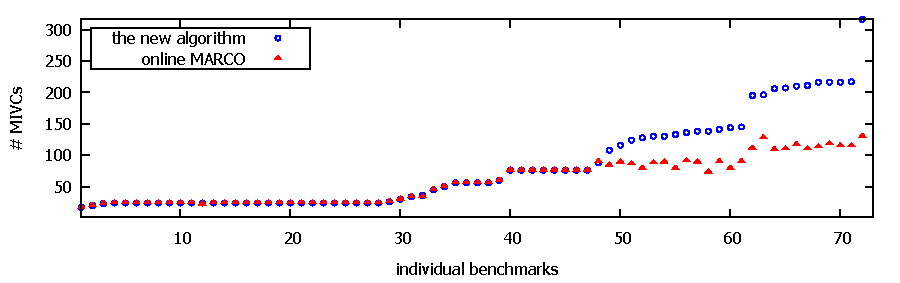
\includegraphics[scale=0.8]{./plots/found_mivcs.pdf}%
\captionof{figure}{Number of MIVCs produced by online algorithms.}%
\label{res:found_mivcs}
\end{minipage}\hfill
\begin{minipage}{.52\textwidth}
\centering
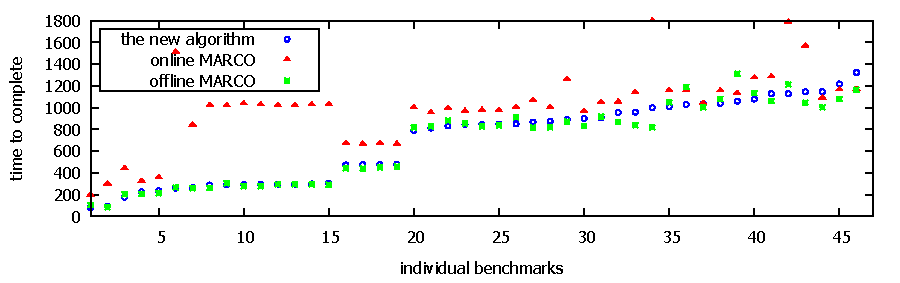
\includegraphics[scale=0.8]{./plots/time_to_complete.pdf}%
\captionof{figure}{Runtime for tractable benchmarks for all algorithms in a log scale.}%
\label{res:time_to_complete}
\end{minipage}
\end{figure}



\subsection{Experimental Results}
In this section, we examine the experimental results to address the research questions.

%\vspace{-5pt}
\paragraph{RQ1 and RQ2:}
Data related to the first two research questions is shown in Figures~\ref{res:found_mivcs} and~\ref{res:time_to_complete}.
Figure~\ref{res:found_mivcs} describes the number of MIVCs found be the two online algorithms in the intractable benchmarks, i.e. the benchmarks where the algorithms did not complete the computation within the time limit. There are 33 such benchmarks.
The Grow-Shrink algorithm substantially outperforms Online MARCO in the majority of the benchmarks, finding an average of 55\% additional MIVCs.

Figure~\ref{res:time_to_complete} describes the time for each algorithm needed to complete the computation in the case of 397 tractable benchmarks. We see that the performance of the Grow-Shrink algorithm is very similar to Offline MARCO, but as previously discussed, has the advantage of returning guaranteed MIVCs, rather than approximate MIVCs.  It is much faster than the Online MARCO algorithm.% which produces MIVCs using MARCO and shrinking.


%\vspace{-5pt}
\paragraph{RQ3:}  For RQ3, we examined the number of required calls to the solver per MIVC.  For this question, we used the 33 models that contained a large number of MIVCs ($>$70) in order to show the solver efficiency as the number of MIVCs increased.  A point with coordinates $(x,y)$ states that the algorithm needed to perform $y$ solver calls (on average) in order to produce (find) the first $x$ MIVCs. We grouped the calls in terms of the number of calls that returned {\em adequate} vs. {\em inadequate} results.  It is evidenced by the results in Figure~\ref{res:checks}, the new algorithm improves upon Online MARCO as the number of MIVCs becomes larger.

\begin{figure}[!t]
\centering
\begin{subfigure}{.5\textwidth}
  \centering
  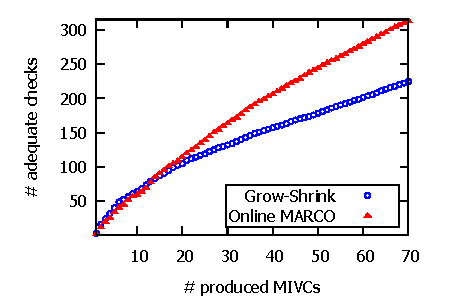
\includegraphics[scale=0.8]{./plots/adequate_checks_per_mivc_70.pdf}
  \caption{Checks with result "adequate".}
  \label{res:adequate_checks}
\end{subfigure}%
\begin{subfigure}{.5\textwidth}
  \centering
  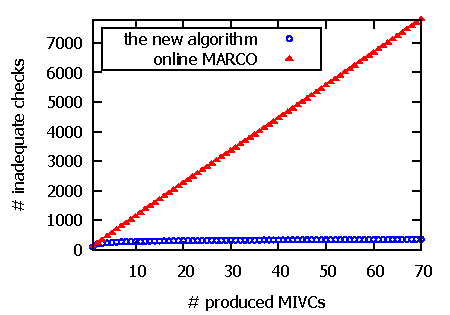
\includegraphics[scale=0.8]{./plots/inadequate_checks_per_mivc_70.pdf}
  \caption{Checks with result "inadequate".}
  \label{res:inadequate_checks}
\end{subfigure}
\caption{Average number of performed adequacy checks required to produce individual MIVCs. Note that Figure (b) is in a log scale.}
\label{res:checks}
\end{figure}

The improvement in the number of \emph{inadequate} calls is due the novel shrinking and growing procedures.
Each (approximately) maximal inadequate subset found by the growing procedure allows to save (up to exponentially) many inadequate calls during subsequent executions of the shrinking procedure.
Indeed, the Grow-Shrink algorithm performed on average only 353 inadequate calls to output the first 70 MIVCs, whereas the online MARCO needed to perform 7775 calls to output the same number of MIVCs.

The improvement in the number of \emph{adequate} calls is not so significant as in the case of inadequate calls. Yet, since the adequate calls are usually much more time consuming than inadequate ones, even a slight saving in the number of adequate calls might significantly speed up the whole computation. The Grow-Shrink algorithm saves adequate calls due to the usage of the shrinking queue and due to the invariants that are maintained by the queue. In particular, shall two comparable sets appear in the queue, only the smaller is left. Thus, the algorithm avoids shrinking of relatively large sets and saves some adequate calls.


\section{Conclusion}
\label{sec:conclusions}
In this paper, we have presented an {\em online} algorithm, called {\em Grow-Shrink algorithm}, for computation of minimal Inductive Validity Cores (MIVCs). The new algorithm substantially outperforms previous approaches.  As opposed to the {\em Offline MARCO} algorithm in~\cite{Ghass17AllIVCs}, it is guaranteed to produce minimal IVCs.  As opposed to a n\"aive extension {\em Online MARCO}, the new algorithm is substantially faster and requires fewer solver calls as the number of MIVCs increases.  We believe that this new algorithm will substantially increase the applicability of software engineering tasks that require MIVCs.  In the future, we hope to examine parallel computation of MIVCs using a variant of this algorithm to further increase scalability.



\bibliographystyle{abbrv}
\bibliography{biblio}


\end{document} 